\newpage 
\section{Numerical Results}

\begin{figure}[H]
    \centering
    \subfigure[]{\includegraphics[width=0.9\textwidth]{Images/13_35x35_ldos.png}}
    \end{figure}
\begin{figure}[H]
    \centering
    \subfigure[]{\includegraphics[width=0.9\textwidth]{Images/13_35x35.png}}
\end{figure}

\begin{figure}[H]
    \centering
    \subfigure[$V= 0.1$]{\includegraphics[width=0.9\textwidth]{Images/gamma_35x35_ldos_V0.1.png}}
    \end{figure}
\begin{figure}[H]
    \centering
    \subfigure[$V=0.1$]{\includegraphics[width=0.9\textwidth]{Images/gamma_35x35_gap.png}}
\end{figure}

\begin{figure}[H]
    \centering
    \subfigure[$V=0.2$]{\includegraphics[width=0.9\textwidth]{Images/gamma_35x35_ldos_V0.2.png}}
    \end{figure}
\begin{figure}[H]
    \centering
    \subfigure[$V=0.2$]{\includegraphics[width=0.9\textwidth]{Images/gamma_35x35_gap_V0.2.png}}
\end{figure}

\begin{figure}[H]
    \centering
    \subfigure[$V= 0.1$, spin 1 in x-direction, spin 2 in y-direction]{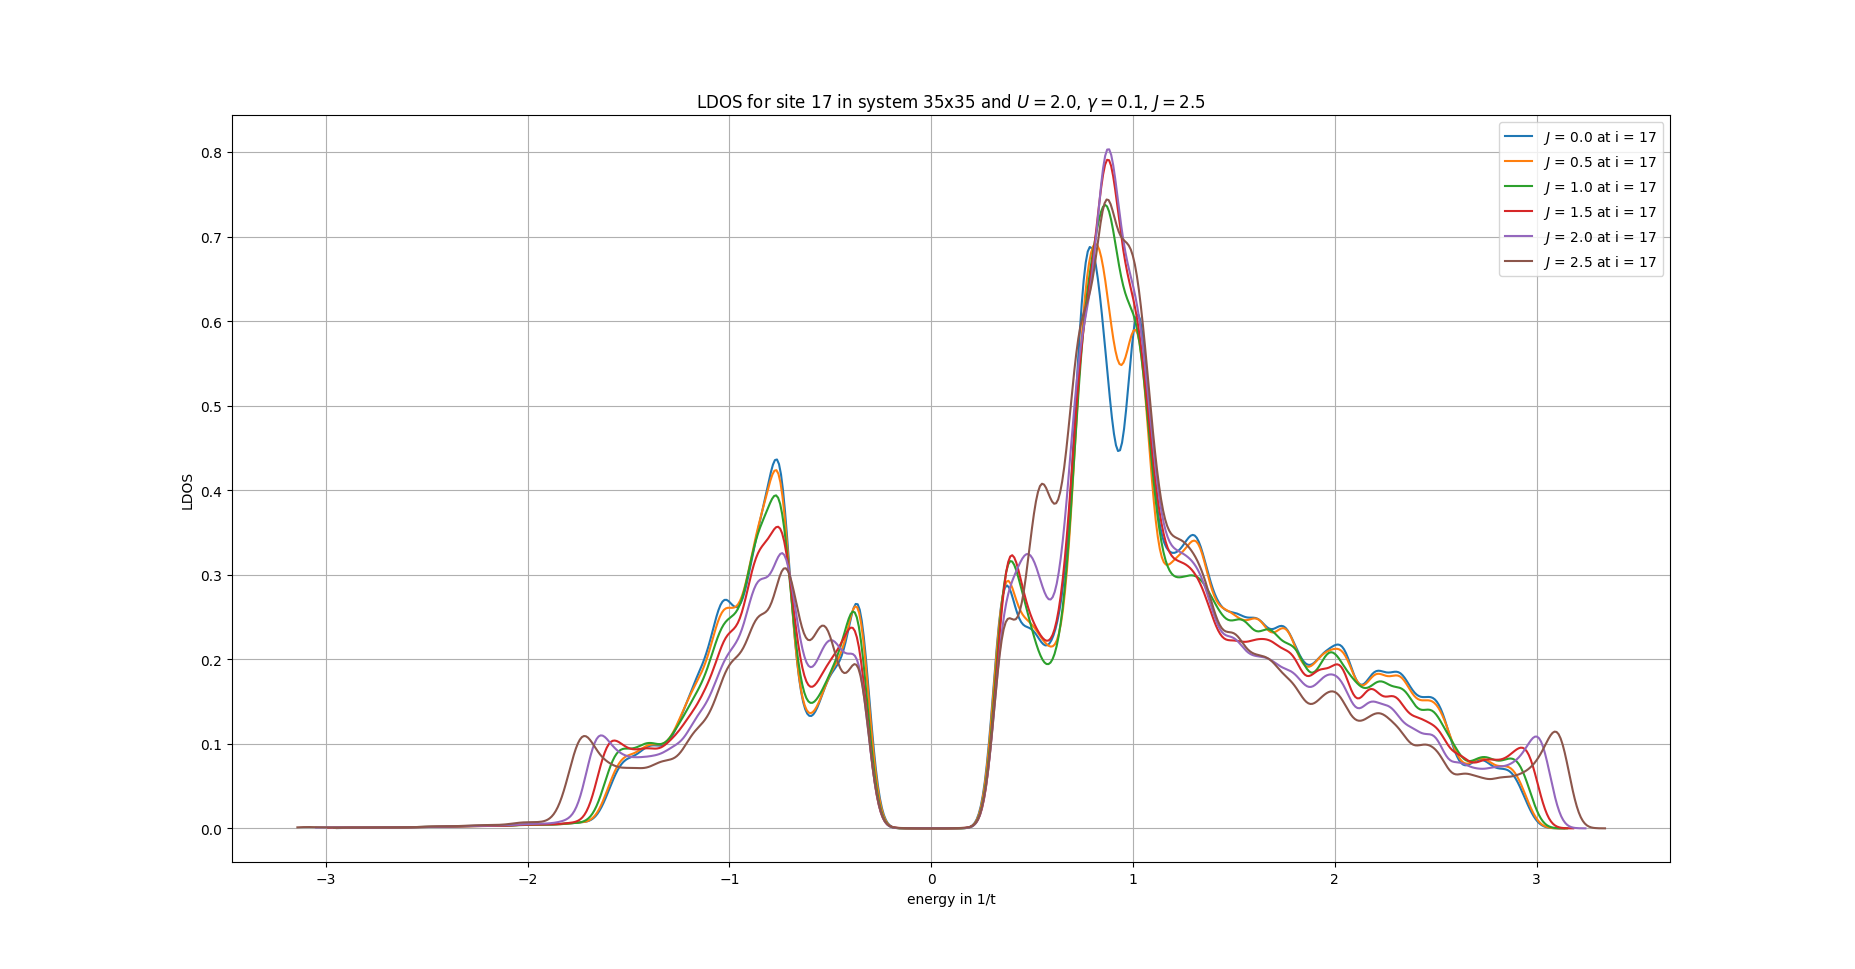
\includegraphics[width=0.9\textwidth]{Images/rkky_35x35_ldos.png}}
    \end{figure}
\begin{figure}[H]
    \centering
    \subfigure[$V= 0.1$, spin 1 in x-direction, spin 2 in y-direction]{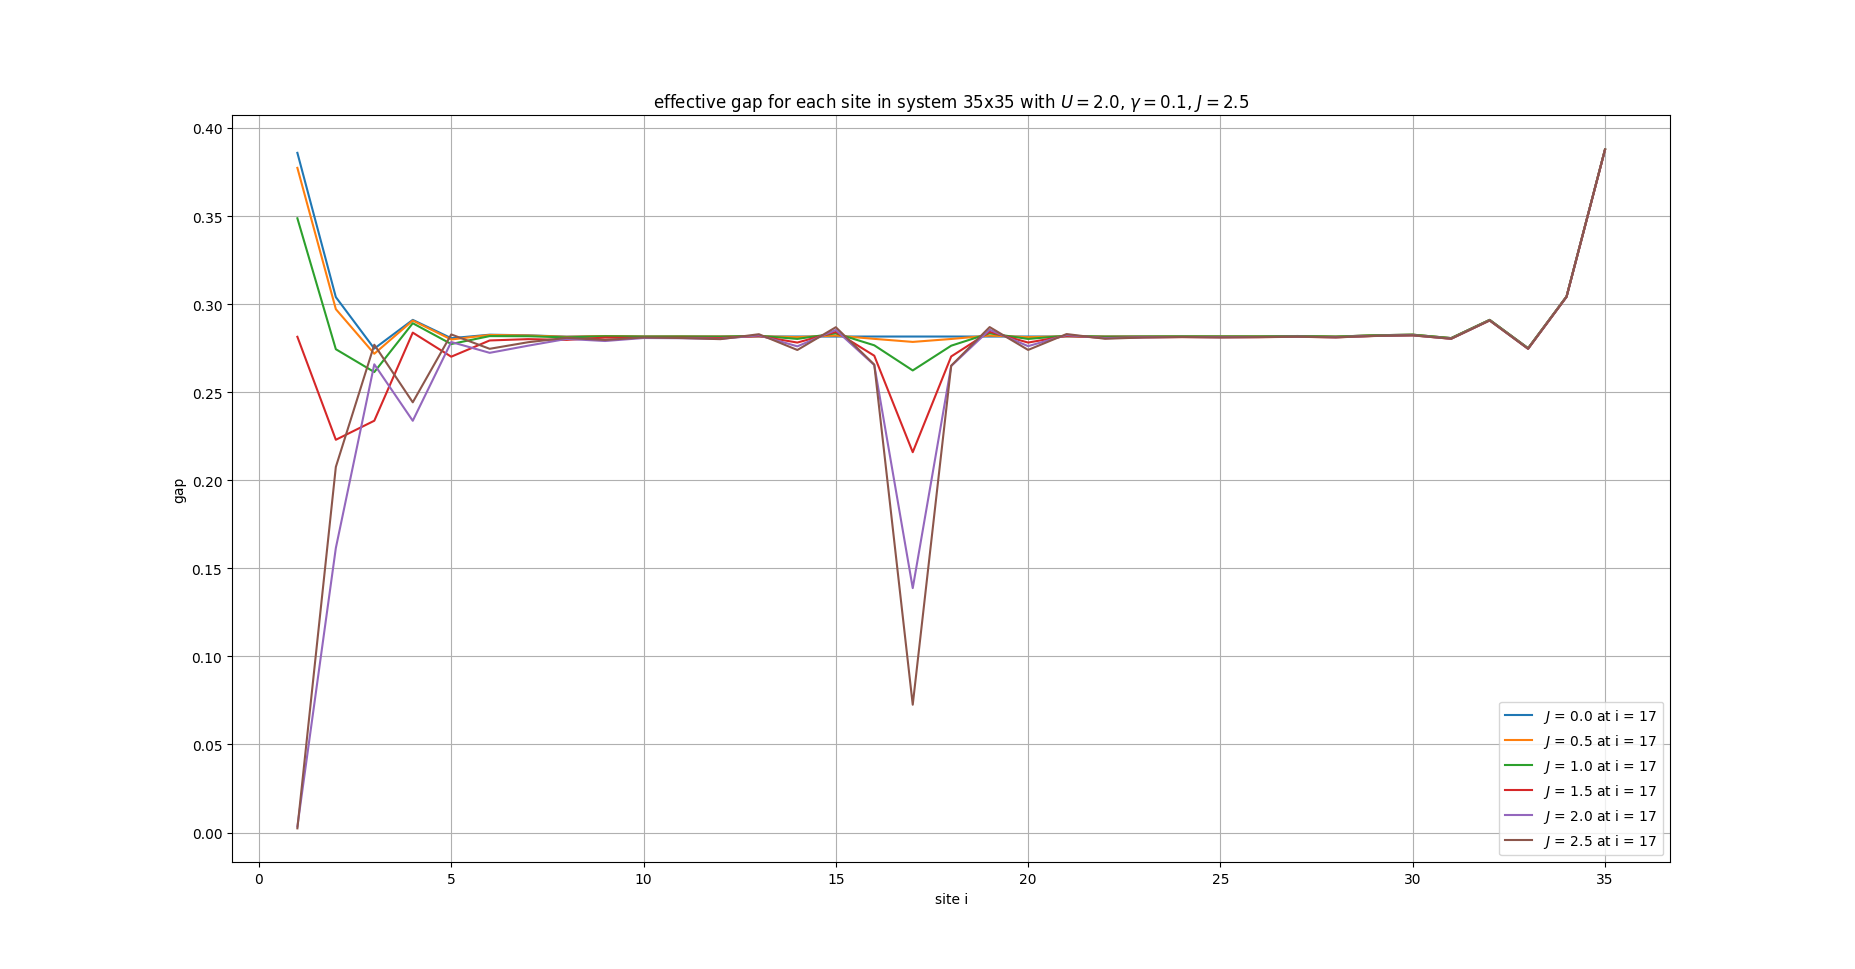
\includegraphics[width=0.9\textwidth]{Images/rkky_35x35_gap.png}}
\end{figure}

\begin{figure}[H]
    \centering
    \subfigure[$V=0.1$, $J=1.5$, spin 1 in x-direction, spin 2 in y-direction]{\includegraphics[width=0.9\textwidth]{Images/gamma_35x35_ldos_V0.1_R1.5.png}}
    \end{figure}
\begin{figure}[H]
    \centering
    \subfigure[$V=0.1$, $J=1.5$, spin 1 in x-direction, spin 2 in y-direction; $\gamma$ enhances the influence of the RKKY interaction on the gap. ]{\includegraphics[width=0.9\textwidth]{Images/gamma_35x35_gap_V0.1_R1.5.png}}
\end{figure}

% \begin{figure}[H]
%     \centering
%     \subfigure[]{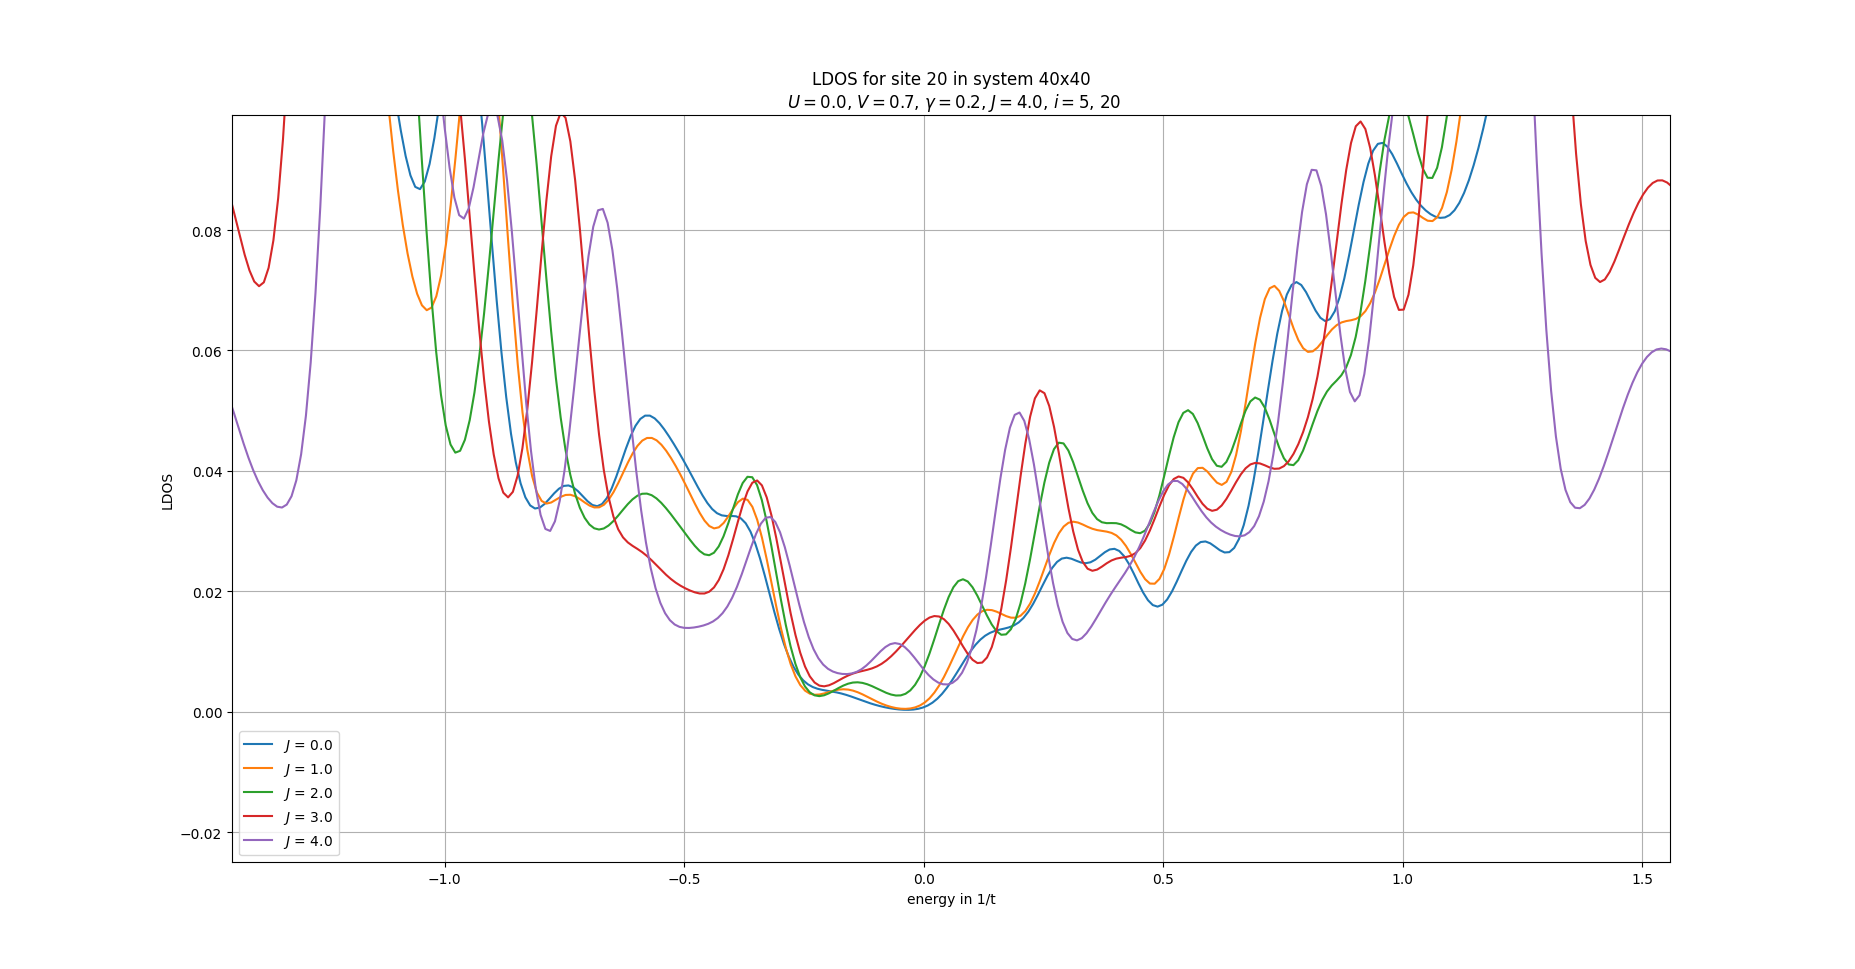
\includegraphics[width=0.48\textwidth]{Images/Figure_1.png}}
%     \subfigure[]{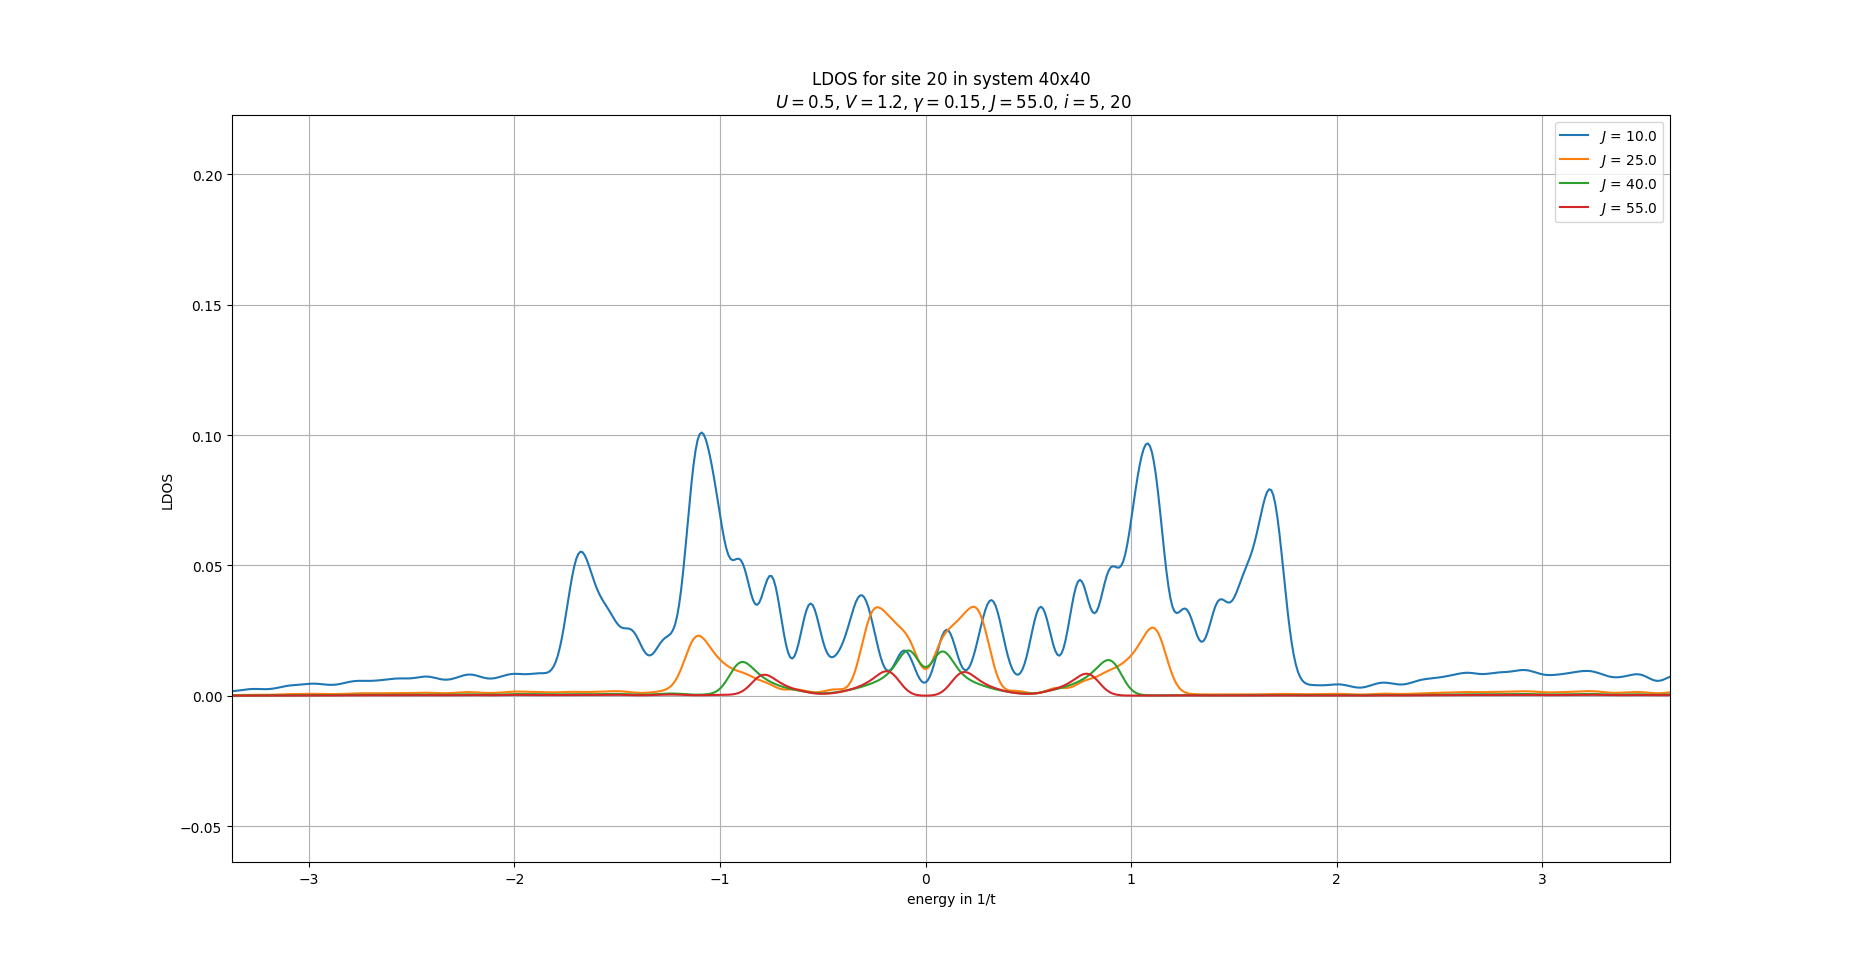
\includegraphics[width=0.48\textwidth]{Images/Figure_2.png}}
% \end{figure}

% \begin{figure}[H]
%     \centering
%     \subfigure[]{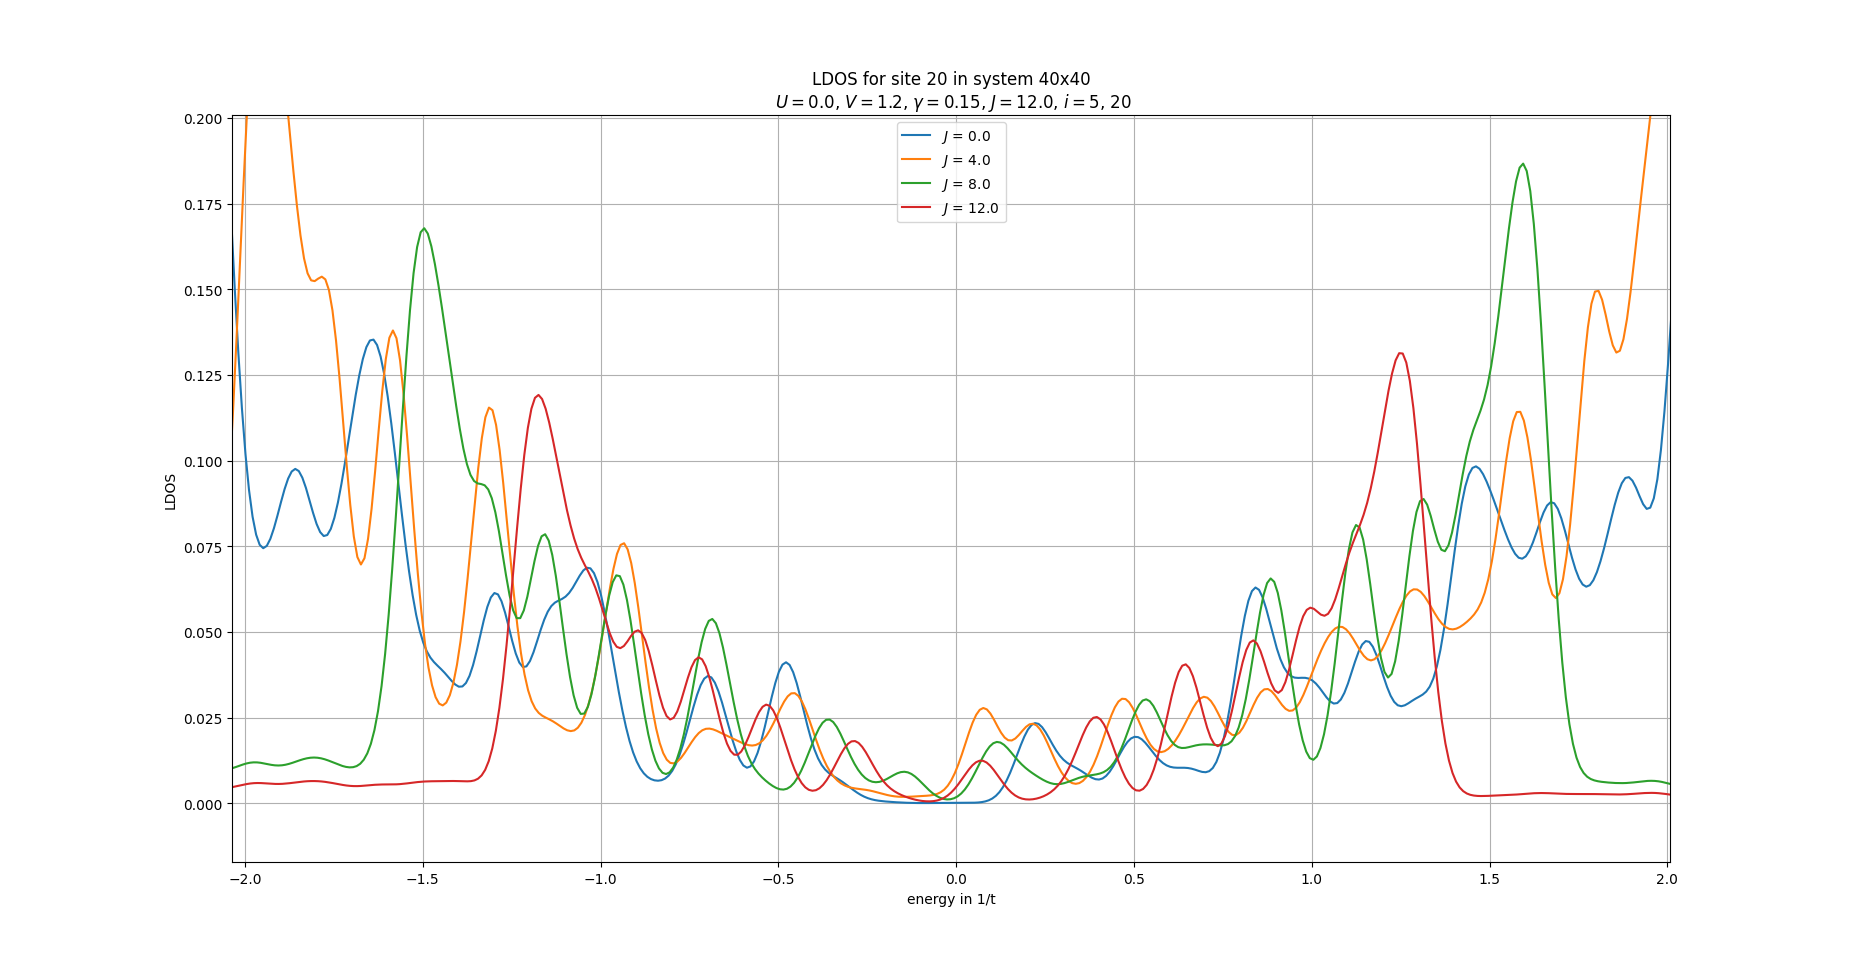
\includegraphics[width=0.48\textwidth]{Images/Figure_3.png}}
%     \subfigure[]{\includegraphics[width=0.48\textwidth]{Images/Figure_4.png}}
% \end{figure}

% \begin{figure}[H]
%     \centering
%     \subfigure[]{\includegraphics[width=0.48\textwidth]{Images/Figure_5.png}}
%     \subfigure[]{\includegraphics[width=0.48\textwidth]{Images/Figure_6.png}}
% \end{figure}

% \begin{figure}[H]
%     \centering
%     \subfigure[]{\includegraphics[width=0.48\textwidth]{Images/Figure_7_fix.png}}
%     \subfigure[]{\includegraphics[width=0.48\textwidth]{Images/Figure_8_fix.png}}
% \end{figure}

% \begin{figure}[H]
%     \centering
%     \subfigure[]{\includegraphics[width=0.48\textwidth]{Images/Figure_7_iteration.png}}
%     \subfigure[]{\includegraphics[width=0.48\textwidth]{Images/Figure_8_iteration.png}}
% \end{figure}
% \begin{figure}[H]
%     \centering
%     \subfigure[]{\includegraphics[width=0.48\textwidth]{Images/ldos_comparison_0gammaJ_mu0.7_F0.png}}
%     \subfigure[100x100]{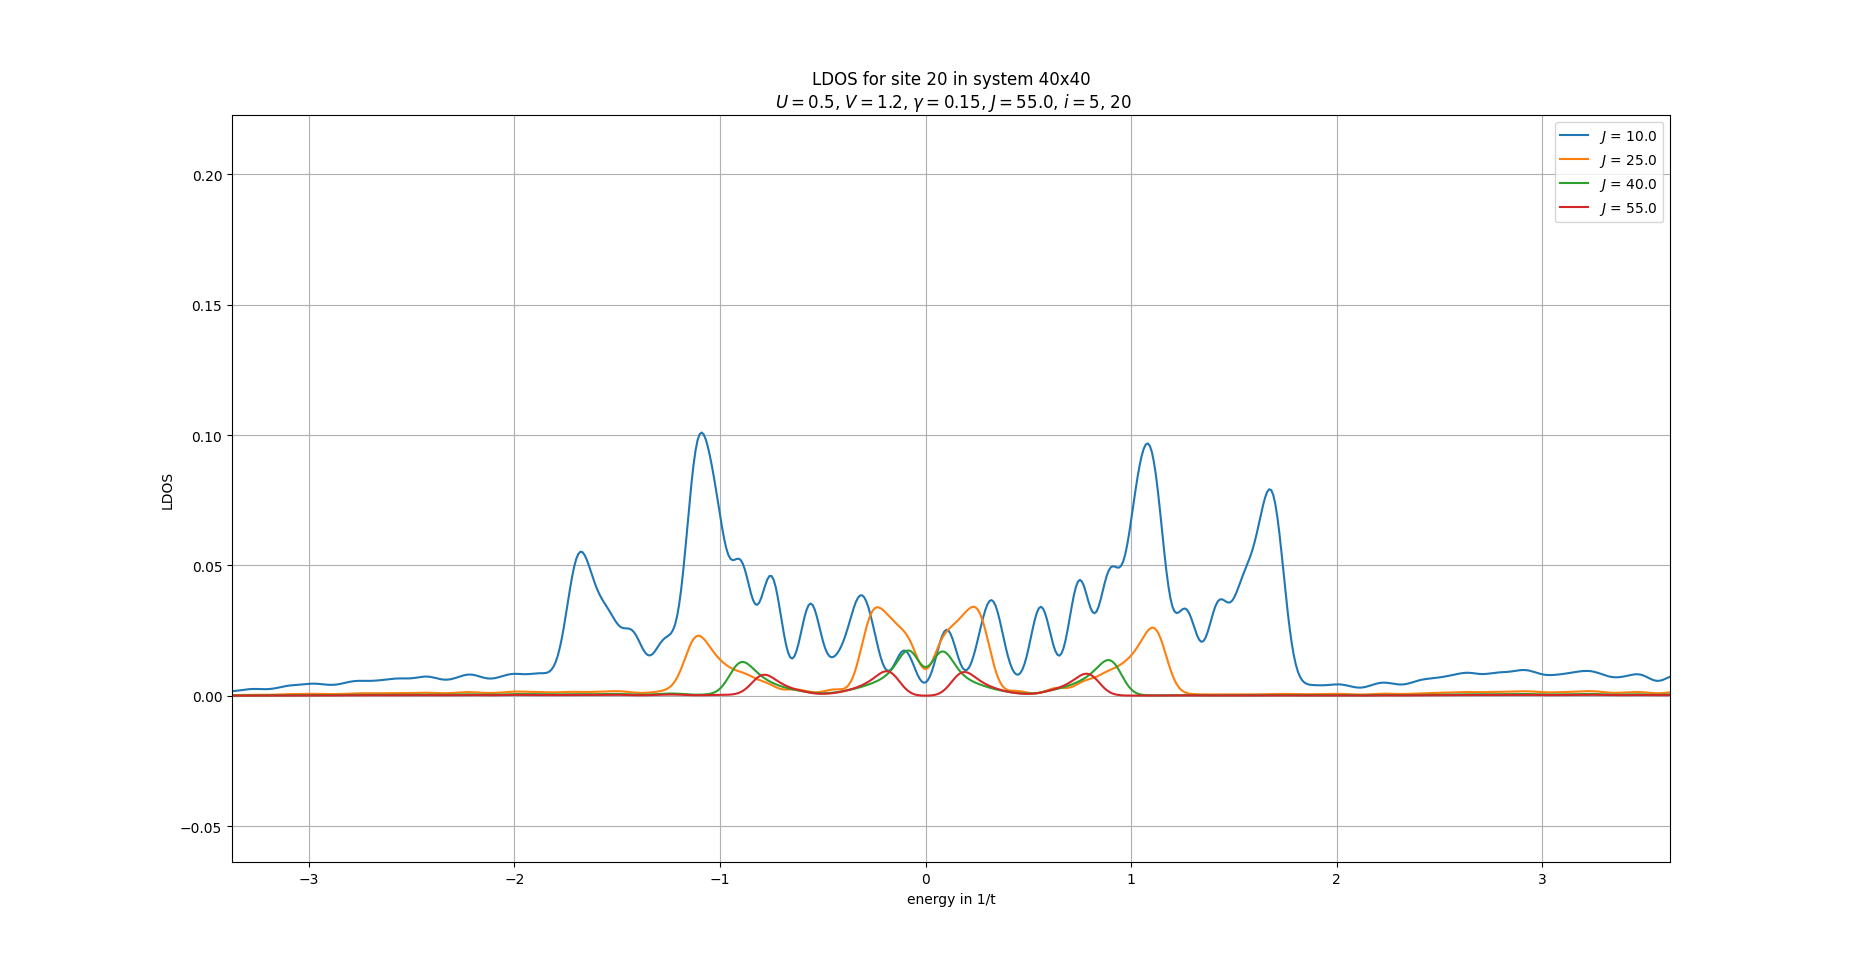
\includegraphics[width=0.48\textwidth]{Images/Figure_2.png}}
% \end{figure}

% \begin{figure}[H]
%     \centering
%     \subfigure[]{\includegraphics[width=0.48\textwidth]{Images/gap_comparison_0gammaJ_mu0.7_F0.png}}
%     \subfigure[100x100]{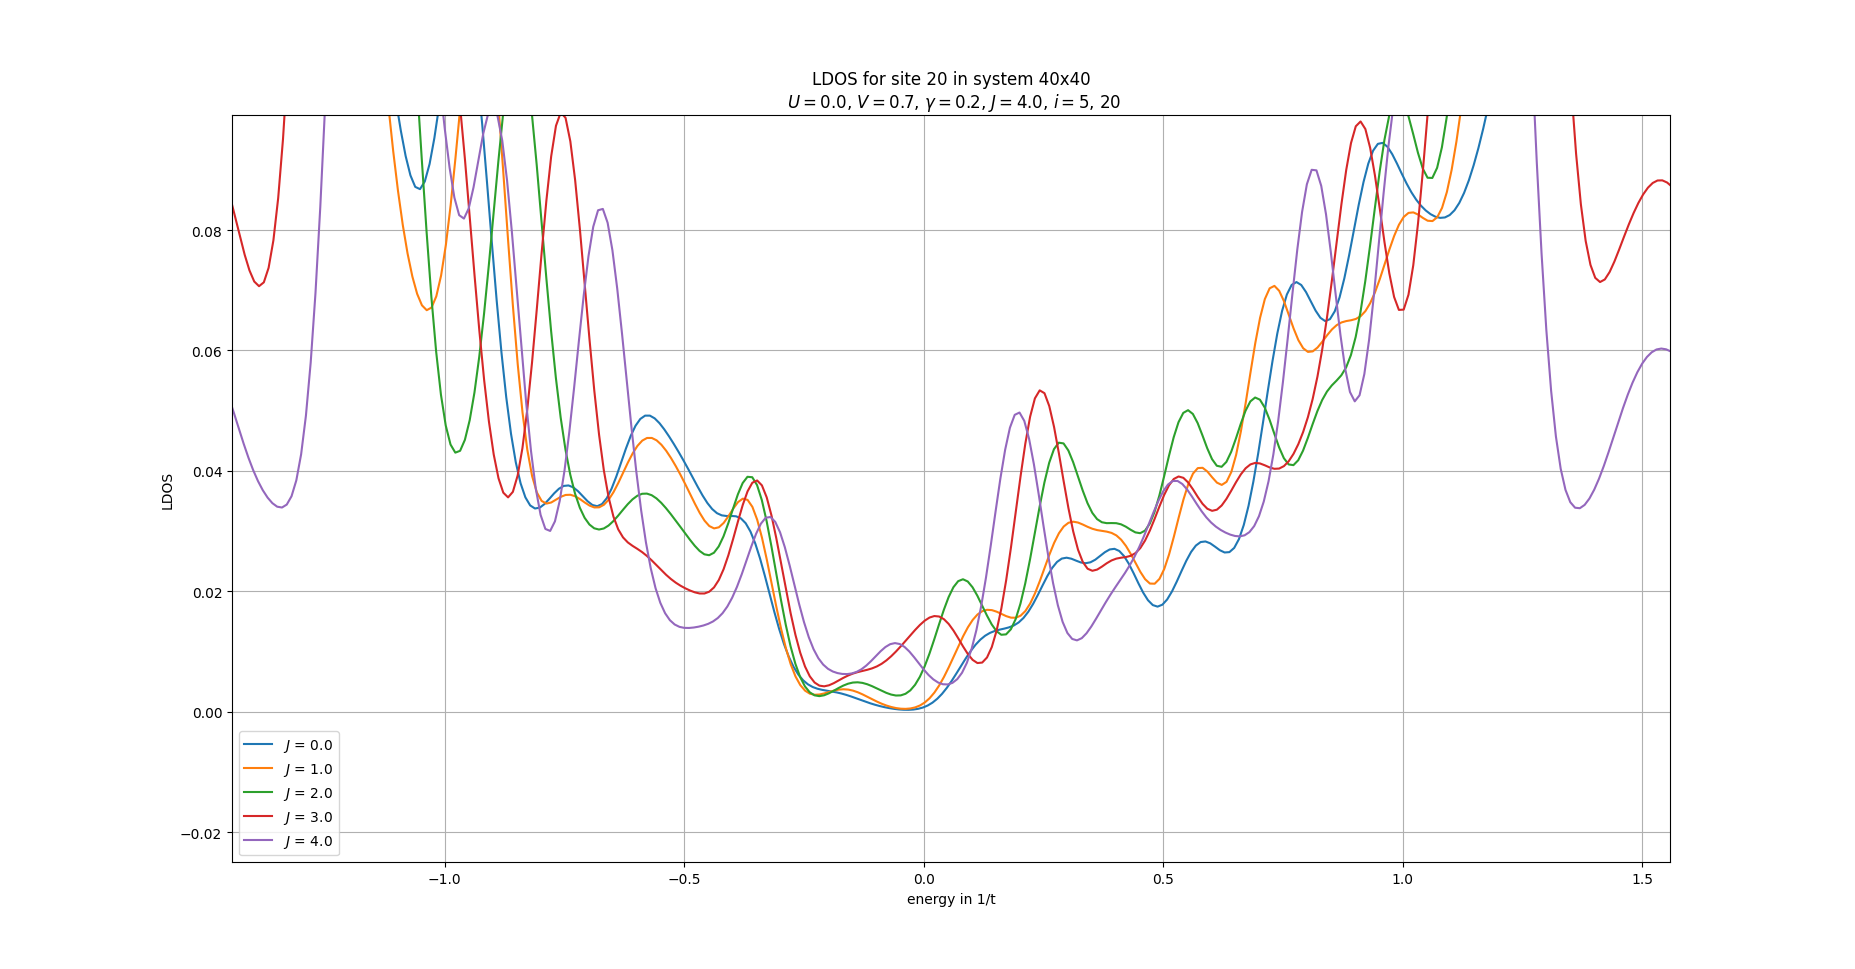
\includegraphics[width=0.48\textwidth]{Images/Figure_1.png}}
% \end{figure}
% the curve does not go significantly up after the sites of impurity.
% \newpage
% \subsection{Gap parameter study}
% \begin{figure}[H]
%     \centering
%     \subfigure[$J=0$]{\includegraphics[width=0.48\textwidth]{Images/parameter_search/gap_comparison_100x100_gamma_mu0.7_V0.png}}
%     \subfigure[$J=1.0$]{\includegraphics[width=0.48\textwidth]{Images/parameter_search/gap_comparison_100x100_Jgamma_mu0.7_V0.png}}
% \end{figure}
% \begin{figure}[H]
%     \centering
%     \subfigure[$\gamma=0$]{\includegraphics[width=0.48\textwidth]{Images/parameter_search/gap_comparison_100x100_J_mu0.7_V0.png}}
%     \subfigure[$\gamma=0.25$]{\includegraphics[width=0.48\textwidth]{Images/parameter_search/gap_comparison_100x100_gammaJ_mu0.7_V0.png}}
% \end{figure}
% \begin{figure}[H]
%     \centering
%     \subfigure[]{\includegraphics[width=0.48\textwidth]{Images/parameter_search/gap_comparison_100x100_U_gamma0.25_V0.png}}
%     \subfigure[]{\includegraphics[width=0.48\textwidth]{Images/parameter_search/gap_comparison_100x100_U_J1.0_V0.png}}
% \end{figure}
% \newpage
% \subsection{LDOS parameter study}
% \begin{figure}[H]
%     \centering
%     \subfigure[$J=0$]{\includegraphics[width=0.48\textwidth]{Images/parameter_search/ldos_comparison_100x100_gamma_mu0.7_V0.png}}
%     \subfigure[$J=1.0$]{\includegraphics[width=0.48\textwidth]{Images/parameter_search/ldos_comparison_100x100_Jgamma_mu0.7_V0.png}}
% \end{figure}
% \begin{figure}[H]
%     \centering
%     \subfigure[$\gamma=0$]{\includegraphics[width=0.48\textwidth]{Images/parameter_search/ldos_comparison_100x100_J_mu0.7_V0.png}}
%     \subfigure[$\gamma=0.25$]{\includegraphics[width=0.48\textwidth]{Images/parameter_search/ldos_comparison_100x100_gammaJ_mu0.7_V0.png}}
% \end{figure}
% \begin{figure}[H]
%     \centering
%     \subfigure[]{\includegraphics[width=0.48\textwidth]{Images/parameter_search/ldos_comparison_100x100_U_gamma0.25_V0.png}}
%     \subfigure[]{\includegraphics[width=0.48\textwidth]{Images/parameter_search/ldos_comparison_100x100_U_J1.0_V0.png}}
% \end{figure}
% \newpage
% \subsection{$\mu$ comparison}

% \begin{figure}[H]
%     \centering
%     \subfigure[]{\includegraphics[width=0.48\textwidth]{Images/parameter_search/gap_comparison_100x100_mu_cps2.0_V0.png}}
%     \subfigure[]{\includegraphics[width=0.48\textwidth]{Images/parameter_search/ldos_comparison_100x100_mu_csp2.0_V0.png}}
% \end{figure}

% % \subsection{Edge States LDOS w/wo Iteration}
% % \begin{figure}
% %     \centering
% %     \includegraphics[width=0.9\textwidth]{Images/comparison_iterationEdgeStates.png}
% %     \caption{30x34, $\mu=0.7$, $U=2.0$, $V,J=0$, $\gamma=0.1$, with and without iteration, first and last four sites in x-direction have U=0}
% %     \label{fig:my_label}
% % \end{figure}
